\documentclass[a4paper,12pt]{report}
\usepackage{mathtext}
\usepackage[T2A]{fontenc}
\usepackage[utf8]{inputenc}
\usepackage[english,russian]{babel}
\usepackage{geometry}
\usepackage{listings}
\usepackage{amsmath}
\geometry{top=2cm}
\usepackage{titlesec}
\usepackage{color}
\usepackage{pgfplots}
\usepackage{filecontents}
\usetikzlibrary{datavisualization}
\usetikzlibrary{datavisualization.formats.functions}
\usepackage{caption}
\DeclareCaptionFont{white}{\color{white}}
\DeclareCaptionFormat{listing}{\colorbox{gray}{\parbox{\textwidth}{#1#2#3}}}
\captionsetup[lstlisting]{format=listing,labelfont=white,textfont=white}

% Для листинга кода:
\lstset{ %
language=C++,                 % выбор языка для подсветки
basicstyle=\small\sffamily, % размер и начертание шрифта для подсветки кода
numbers=left,               % где поставить нумерацию строк (слева\справа)
numberstyle=\tiny,           % размер шрифта для номеров строк
stepnumber=1,                   % размер шага между двумя номерами строк
numbersep=-5pt,                % как далеко отстоят номера строк от подсвечиваемого кода
showspaces=false,
backgroundcolor=\color{white},         
showstringspaces=false,      % показывать или нет пробелы в строках
showtabs=false,             % показывать или нет табуляцию в строках
frame=single,              % рисовать рамку вокруг кода
tabsize=2,                 % размер табуляции по умолчанию равен 2 пробелам
captionpos=t,              % позиция заголовка вверху [t] или внизу [b] 
breaklines=true,           % автоматически переносить строки (да\нет)
breakatwhitespace=false, % переносить строки только если есть пробел
escapeinside={\%*}{*)},   % если нужно добавить комментарии в коде
	    keywordstyle=\color{blue}\ttfamily,
	    stringstyle=\color{red}\ttfamily,
	    commentstyle=\color{green}\ttfamily,
	    morecomment=[l][\color{magenta}]{\#},
	    columns=fullflexible   % если нужно добавить комментарии в коде
}

% Для измененных титулов глав:
\definecolor{gray75}{gray}{0.75} % определяем цвет
\newcommand{\hsp}{\hspace{20pt}} % длина линии в 20pt
% titleformat определяет стиль
\titleformat{\chapter}[hang]{\Huge\bfseries}{\thechapter\hsp\textcolor{gray75}{|}\hsp}{0pt}{\Huge\bfseries}


% Графики
\begin{filecontents}{VinogradEven.dat}
100 9.9327
200 79.7351
300 277.48
400 727.771
500 1393.57
600 2429.5
700 4031.91
800 6104.68
900 15963.7
1000 20571.1
\end{filecontents}

\begin{filecontents}{x2ThreadedEven.dat}
100 5.5233
200 37.6127
300 131.876
400 340.379
500 678.334
600 1152.39
700 1913.31
800 2928.91
900 5259.16
1000 9766.11
\end{filecontents}

\begin{filecontents}{x4ThreadedEven.dat}
100 4.0258
200 22.4721
300 74.0728
400 192.715
500 366.086
600 648.897
700 1075.4
800 1587.02
900 3170.67
1000 4762.84
\end{filecontents}

\begin{filecontents}{x8ThreadedEven.dat}
100 4.3916
200 22.819
300 70.2347
400 176.775
500 347.213
600 574.199
700 921.204
800 1372.61
900 2531.54
1000 3721.84
\end{filecontents}

\begin{filecontents}{VinogradOdd.dat}
101 10.4512
201 77.4892
301 273.502
401 737.146
501 1550.06
601 2551.18
701 4209.71
801 6488.39
901 10213.8
1001 14802.7
\end{filecontents}

\begin{filecontents}{x2ThreadedOdd.dat}
101 5.545
201 37.0545
301 130.254
401 343.22
501 700.715
601 1186.33
701 2091.4
801 3112.45
901 5844.36
1001 9016.48
\end{filecontents}

\begin{filecontents}{x4ThreadedOdd.dat}
101 4.144
201 20.6978
301 75.2233
401 193.633
501 391.185
601 655.233
701 1226.77
801 1661.57
901 3541.88
1001 4810.92
\end{filecontents}

\begin{filecontents}{x8ThreadedOdd.dat}
101 4.7815
201 23.0499
301 70.2161
401 189.404
501 352.557
601 588.748
701 1036.58
801 1458.22
901 2799.61
1001 3938.15
\end{filecontents}


\begin{document}
\begin{titlepage}
	\centering
	{\scshape\LARGE МГТУ им. Н.Э.Баумана \par}
	\vspace{4cm}
	{\scshape\Large Лабораторная работа №2\par}
	\vspace{0.5cm}	
	{\scshape\Large По курсу: "Анализ алгоритмов"\par}
	\vspace{2cm}
	{\huge\bfseries Параллельное умножение матриц\par}
	\vspace{3cm}
	\Large Работу выполнил: Луговой Дмитрий, ИУ7-51Б\par
	\vspace{0.5cm}
	\Large Преподаватель:  Волкова Л.Л.\par

	\vfill
	\large \textit {Москва, 2019} \par
\end{titlepage}

\setcounter{page}{2}

\tableofcontents

\newpage
\chapter*{Введение}
\addcontentsline{toc}{chapter}{Введение}
\hspace{0.6cm} \textbf{Цель работы}: изучение возможности параллельных вычислений и использование такого подхода на практике. Реализация параллельного алгоритма Винограда умножения матриц. 
В данной лабораторной работе рассматривается алгоритм Винограда и параллельный алгоритм Винограда. Необходимо сравнить зависимость времени работы алгоритма от числа параллельных потоков и размера матриц, провести сравнение стандартного и параллельного алгоритмов.\\\\

\textbf{\LARGE Задачи работы}\\\\
Задачами данной лабораторной являются:
\begin{enumerate}
\item[1)] Научиться писать многопоточные программы;
\item[2)] Применить полученные знания на практике, переписав алгоритм Винограда в несколько потоков;
\item[3)] Провести замеры скорости работы однопоточной и многопоточной реализаций и проанализировать полученные результаты.
\end{enumerate}


\chapter{Аналитическая часть}
\hspace{0.6cm}В данном разделе содержатся описание алгоритма Винограда умножения матриц, определение потока и многопоточного программирования.

\section{Стандартный алгоритм}
\hspace{0.6cm}Пусть даны две прямоугольные матрицы A и B размерностей $m \times n$ , $n \times q$ соответственно:

\[
A = 
  \begin{bmatrix} 
    a_{11} & a_{12} & \cdots & a_{1n} \\
    a_{21} & a_{22} & \cdots & a_{2n} \\ 
    \vdots & \vdots & \ddots & \vdots \\ 
    a_{m1} & a_{m2} & \cdots & a_{mn}
  \end{bmatrix},\;\;\;
\]
\[
B =   
  \begin{bmatrix} 
    b_{11} & b_{12} & \cdots & b_{1q} \\
    b_{21} & b_{22} & \cdots & b_{2q} \\ 
    \vdots & \vdots & \ddots & \vdots \\ 
    b_{n1} & b_{n2} & \cdots & b_{nq}.
  \end{bmatrix}.
\]
Тогда матрица C размерностью $m \times q$
\[
C = 
  \begin{bmatrix} 
    c_{11} & c_{12} & \cdots & c_{1q} \\
    c_{21} & c_{22} & \cdots & c_{2q} \\ 
    \vdots & \vdots & \ddots & \vdots \\ 
    c_{m1} & c_{m2} & \cdots & c_{mq}
  \end{bmatrix},
\]
в которой:\\

$c_{ij} = \sum_{k=1}^n a_{ik}b_{kj} \;\;\; \left(i=1, 2, \ldots m;\; j=1, 2, \ldots q \right)$\\

называется их произведением. Операция умножения двух матриц выполнима только в том случае, если число столбцов в первом сомножителе равно числу строк во втором; в этом случае говорят, что матрицы согласованы. В частности, умножение всегда выполнимо, если оба сомножителя — [[Квадратная матрица|квадратная матрица]] одного и того же порядка. 

Таким образом, из существования произведения AB вовсе не следует существование произведения BA

\section{Алгоритм Винограда}
\hspace{0.6cm} \textbf {Алгоритм Винограда} — алгоритм умножения матриц, предложенный в 1987 году Ш. Виноградом. В исходной версии асимптотическая сложность алгоритма составляла $O(n^{2,3755})$, где n — размер стороны матрицы. Алгоритм Винограда, с учетом серии улучшений и доработок в последующие годы, обладает лучшей асимптотикой среди известных алгоритмов умножения матриц.\\
Если посмотреть на результат умножения двух матриц, то видно, что каждый элемент в нем представляет собой скалярное произведение соответствующих строки и столбца исходных матриц. Можно заметить также, что такое умножение допускает предварительную обработку, позволяющую часть работы выполнить заранее. 
Рассмотрим два вектора
$V = (v1, v2, v3, v4)$ и
$W = (w1, w2, w3, w4)$.
Их скалярное произведение равно: 
$V * W = v1w1 + v2w2 + v3w3 + v4w4$.
Это равенство можно переписать в виде: 
$V * W = (v1 + w2)(v2 + w1) + (v3 + w4)(v4 + w3) - v1v2 - v3v4 - w1w2 - w3w4$.

Кажется, что второе выражение задает больше работы, чем первое: вместо четырех умножений мы насчитываем их шесть, а вместо трех сложений - десять. Однако выражение в правой части последнего равенства допускает предварительную обработку: его части можно вычислить заранее и запомнить для каждой строки первой матрицы и для каждого столбца второй. На практике это означает, что над предварительно обработанными элементами нам придется выполнять лишь первые два умножения и последующие пять сложений, а также дополнительно два сложения.

\section{Многопоточность}
\hspace{0.6cm} \textbf {Поток выполнения} — наименьшая единица обработки, исполнение которой может быть назначено ядром операционной системы. Реализация потоков выполнения и процессов в разных операционных системах отличается друг от друга, но в большинстве случаев поток выполнения находится внутри процесса. Несколько потоков выполнения могут существовать в рамках одного и того же процесса и совместно использовать ресурсы, такие как память, тогда как процессы не разделяют этих ресурсов. В частности, потоки выполнения разделяют инструкции процесса (его код) и его контекст (значения переменных, которые они имеют в любой момент времени).

На одном процессоре многопоточность обычно происходит путём временного мультиплексирования (как и в случае многозадачности): процессор переключается между разными потоками выполнения. Это переключение контекста обычно происходит достаточно часто, чтобы пользователь воспринимал выполнение потоков или задач как одновременное. В многопроцессорных и многоядерных системах потоки или задачи могут реально выполняться одновременно, при этом каждый процессор или ядро обрабатывает отдельный поток или задачу.

Потоки возникли в операционных системах как средство распараллеливания вычислений.

Параллельное выполнение нескольких работ в рамках одного интерактивного приложения повышает эффективность работы пользователя. Так, при работе с текстовым редактором желательно иметь возможность совмещать набор нового текста с такими продолжительными по времени операциями, как переформатирование значительной части текста, печать документа или его сохранение на локальном или удаленном диске. Еще одним примером необходимости распараллеливания является сетевой сервер баз данных. В этом случае параллелизм желателен как для обслуживания различных запросов к базе данных, так и для более быстрого выполнения отдельного запроса за счет одновременного просмотра различных записей базы. Именно для этих целей современные ОС предлагают механизм многопоточной обработки (multithreading). Понятию «поток» соответствует последовательный переход процессора от одной команды программы к другой. ОС распределяет процессорное время между потоками. Процессу ОС назначает адресное пространство и набор ресурсов, которые совместно используются всеми его потоками. 

Создание потоков требует от ОС меньших накладных расходов, чем процессов. В отличие от процессов, которые принадлежат разным, вообще говоря, конкурирующим приложениям, все потоки одного процесса всегда принадлежат одному приложению, поэтому ОС изолирует потоки в гораздо меньшей степени, нежели процессы в традиционной мультипрограммной системе. Все потоки одного процесса используют общие файлы, таймеры, устройства, одну и ту же область оперативной памяти, одно и то же адресное пространство. Это означает, что они разделяют одни и те же глобальные переменные. Поскольку каждый поток может иметь доступ к любому виртуальному адресу процесса, один поток может использовать стек другого потока. Между потоками одного процесса нет полной защиты, потому что, во-первых, это невозможно, а во-вторых, не нужно. Чтобы организовать взаимодействие и обмен данными, потокам вовсе не требуется обращаться к ОС, им достаточно использовать общую память — один поток записывает данные, а другой читает их. С другой стороны, потоки разных процессов по-прежнему хорошо защищены друг от друга.

\chapter{Конструкторская часть}
\hspace{0.6cm}В этом разделе содержится cхема алгоритма Винограда умножения матриц и описание распараллеливания этого алгоритма.
\newpage
\section{Схемы алгоритмов}

На Рис.2.1, 2.2, 2.3 и 2.4 представлена схема оптимизированного алгоритма Винограда умножения матриц.

\begin{figure}[ht!]
\center{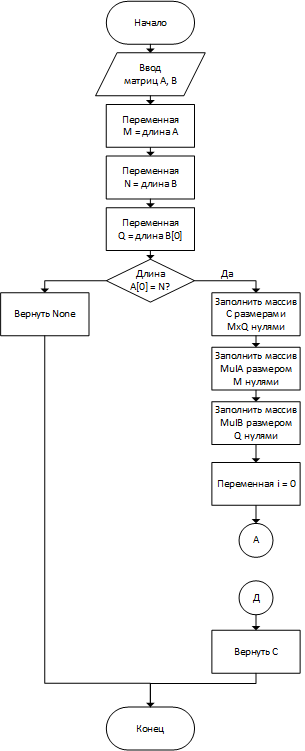
\includegraphics[scale=1]{Optimized1.png}}
\caption{Алгоритм Винограда умножения матриц}
\end{figure}

\newpage

\begin{figure}[ht!]
\center{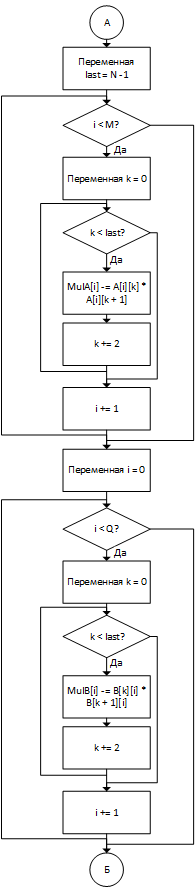
\includegraphics[scale=0.9]{Optimized2.png}}
\caption{Алгоритм Винограда умножения матриц(продолжение 1)}
\end{figure}

\newpage

\begin{figure}[ht!]
\center{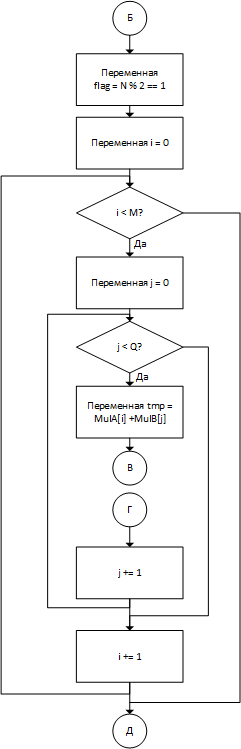
\includegraphics[scale=1]{Optimized3.png}}
\caption{Алгоритм Винограда умножения матриц(продолжение 2)}
\end{figure}

\newpage

\begin{figure}[ht!]
\center{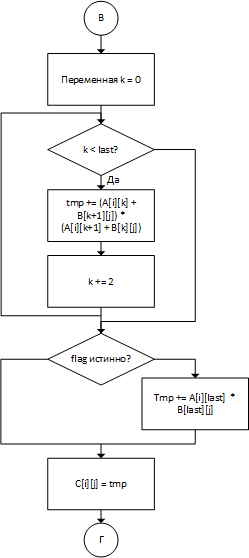
\includegraphics[scale=1]{Optimized4.png}}
\caption{Алгоритм Винограда умножения матриц(продолжение 3)}
\end{figure}

\section{Распараллеливание программы}
Распараллеливание программы должно ускорять время работы. Это достигается за счет реализации в узких участках (например в циклах с большим количеством независимых вычислений).

В предложенном алгоритме данными участками  являются тройной цикл поиска результата(участок от Б до Д), цикл вычисления сумм перемноженных пар строк первой матрицы и  сумм перемноженных пар столбцов второй матрицы(участок от А до Б).

Данные участки программы как раз предлагается распараллелить.

\section{Вывод}
Была приведена схема алгоритма Винограда и выявлены участки программы, которые могут быть распараллелены. 

\chapter{Технологическая часть}
\hspace{0.6cm}В данном разделе приведены требования к программному обеспечению, средства реализации и листинги кода
\section{Требования к ПО}

\hspace{0.6cm}На вход поступают две целочисленные матрицы, на выходе должен возвращаться результат их умножения и код завершения.
	
\section{Средства реализации}
\hspace{0.6cm}Для реализации представленных алгоритмов был выбран язык C++. Время работы алгоритмов было замерено с помощью функции steady\_clock() из библиотеки chrono. Для тестирования использовался компьютер на базе процессора Intel Core i5 (4 физических ядра, 8 логических).

\section{Листинги кода}

\hspace{0.6cm}В Листинге 3.1 показана реализация алгоритма Винограда умножения матриц.

\begin{lstlisting}[caption=Функция умножения матриц алгоритмом Винограда]
  int vinograd(std::vector<std::vector<int>> &C,  const ::vector<std::vector<int>> &A,
          const std::vector<std::vector<int>> &B)
  {
      int m = A.size();
      int n = B.size();
      if (m == 0 || n == 0)
          return ERR_EMPTY;
      if (A[0].size() != n)
          return ERR_SIZE;
      int q = B[0].size();
      std::vector<int> mulA(m,0);
      for (int i = 0; i < m; i++)
      {
          for (int j = 0; j < n - 1; j += 2)
          {
              mulA[i] -= A[i][j] * A[i][j + 1];
          }
      }
      std::vector<int> mulB(q,0);
      for (int i = 0; i < q; i++)
      {
          for (int j = 0; j < n - 1; j += 2)
          {
              mulB[i] -= B[j][i] * B[j + 1][i];
          }
      }
      int last = n - 1;
      bool flag = n % 2 == 1;
      C = std::vector<std::vector<int>> (m, std::vector<int> (q, 0));
      for (int i = 0; i < m; i++)
      {
          for (int j = 0; j < q; j++)
          {
              int tmp = mulA[i] + mulB[j];
              for (int k = 0; k < n - 1; k += 2)
              {
                  tmp += (A[i][k] + B[k + 1][j]) * (A[i][k + 1] + B[k][j]);
              }
              if (flag)
              {
                  tmp += A[i][last] * B[last][j];
              }
              C[i][j] = tmp;
          }
      }
      return OK;
  }
\end{lstlisting}

В Листингах 3.2, 3.3, 3.4. 3.5 показана реализация многопоточного алгоритма Винограда умножения матриц.
\begin{lstlisting}[caption=Функция умножения матриц многопоточным алгоритмом Винограда]
  int threadedVinograd(std::vector<std::vector<int>> &C, const std::vector<std::vector<int>> &A,
               const std::vector<std::vector<int>> &B, const int &nThreads)
  {
      int m = A.size();
      int n = B.size();
      if (m == 0 || n == 0)
          return ERR_EMPTY;
      if (A[0].size() != n)
          return ERR_SIZE;
      int q = B[0].size();
      std::vector<std::thread> threads;
      std::vector<int> mulA(m,0);
      double start = 0;
      double del = m / static_cast<double>(nThreads);
      for (int i = 0; i < nThreads; i++)
      {
          threads.push_back(std::thread(computeMulA, std::ref(mulA), A, round(start),
                                        round(start + del)));
          start += del;
      }
      for (auto &thread: threads)
      {
          thread.join();
      }
      start = 0;
      del = q / static_cast<double>(nThreads);
      std::vector<int> mulB(q,0);
      for (int i = 0; i < nThreads; i++)
      {
          threads[i] = std::thread(computeMulB, std::ref(mulB), B,
                                   round(start), round(start + del));
          start += del;
      }
      for (auto &thread: threads)
      {
          thread.join();
      }

      C = std::vector<std::vector<int>> (m, std::vector<int> (q, 0));
      start = 0;
      del = m / static_cast<double>(nThreads);
      for (int i = 0; i < nThreads; i++)
      {
          threads[i] = std::thread(computeResult, std::ref(C), A, B,
                                   mulA, mulB, round(start), round(start + del));
          start += del;
      }
      for (auto &thread: threads)
      {
          thread.join();
      }
      return OK;
  }
\end{lstlisting}

\begin{lstlisting}[caption=Функция вычисления сумм строк первой матрицы]
  void computeMulA(std::vector<int> &mulA, std::vector<std::vector<int>> A, int startRow, int endRow)
  {
      int n = A[0].size();
      for (int i = startRow; i < endRow; i++)
      {
          for (int j = 0; j < n - 1; j += 2)
          {
              mulA[i] -= A[i][j] * A[i][j + 1];
          }
      }
  }
\end{lstlisting}

\begin{lstlisting}[caption=Функция вычисления сумм столбцов второй матрицы]
  void computeMulB(std::vector<int> &mulB, std::vector<std::vector<int>> B, int startCol, int endCol)
  {
      int n = B.size();
      for (int i = startCol; i < endCol; i++)
      {
          for (int j = 0; j < n - 1; j += 2)
          {
              mulB[i] -= B[j][i] * B[j + 1][i];
          }
     }
  }
\end{lstlisting}

\begin{lstlisting}[caption=Функция вычисления результирующей матрицы]
  void computeResult(std::vector<std::vector<int>> &C, std::vector<std::vector<int>> A,
                     std::vector<std::vector<int>> B, std::vector<int> mulA,
                     std::vector<int> mulB, int startRow, int endRow)
  {
      int n = B.size();
      int q = B[0].size();
      int last = n - 1;
      bool flag = n % 2 == 1;
      for (int i = startRow; i < endRow; i++)
      {
          for (int j = 0; j < q; j++)
          {
              int tmp = mulA[i] + mulB[j];
              for (int k = 0; k < n - 1; k += 2)
              {
                  tmp += (A[i][k] + B[k + 1][j]) * (A[i][k + 1] + B[k][j]);
              }
              if (flag)
              {
                  tmp += A[i][last] * B[last][j];
              }
              C[i][j] = tmp;
          }
      }
  }
\end{lstlisting}
\

\chapter{Экспериментальная часть}
В данном разделе приведены примеры работы программы, постановка эксперимента и сравнительный анализ алгоритмов на основе экспериментальных данных.
\section{Примеры работы}
\hspace{0.6cm}\textbf {Пример 1}\\
Матрица A:\\
1 2 3\\
4 5 6\\
Матрица B:\\
1\\
2\\
3\\
Результирующая матрица:\\
14\\
32\\

\textbf {Пример 2}\\
Матрица A:\\
5 2\\
1 4\\
Матрица B:\\\
0 3\\
-6 1\\
Результирующая матрица:\\
-12 17\\
-24 7\\

\newpage 
\textbf {Пример 3}\\
Матрица A:\\
2 7\\
1 3\\
Матрица B:\\
-3 7\\
1 -2\\
Результирующая матрица:\\
1 0\\
0 1\\

\section{Функциональное тестирование}
\hspace{0.6cm}Было проведено функциональное тестирование программы, результаты которого занесены в Таблицу 4.1,1 столбец которой - номер тестового случая, 2 и 3 столбцы - виды матриц, поступающих на вход, 4 столбец - ожидаемый результат, 5 столбец - полученный результат. \\

\begin{table}[h!]
\begin{center}
\begin{tabular}{| c | c | c | c | c |}
\hline
№ & A & B & Ожидаемый результат & Полученный результат \\
\hline
1 & Случайная & Пустая & Код ошибки &  Код ошибки\\
\hline
2 & Пустая & Случайная &  Код ошибки &  Код ошибки\\
\hline
3 & Пустая & Пустая &  Код ошибки &  Код ошибки\\
\hline
4 & Случайная & Нулевая & Нулевая & Нулевая\\
\hline
5 & Нулевая & Случайная & Нулевая  & Нулевая \\
\hline
6 & Единичная & Квадратная & B & B\\
\hline
7 & Квадратная & Единичная & A & A\\
\hline
8 & Размера $M \times N$ & Размера $M \times N$ &  Код ошибки &  Код ошибки\\
\hline
\end{tabular}
\caption{Тестовые случаи}
\end{center}
\end{table}

Программа успешно прошла все тестовые случаи, все полученные результаты совпали с ожидаемыми.

\section{Сравение алгоритмов по времени}
\hspace{0.6cm}Для экспериментов использовались матрицы, размер которых варьируется от $100 \times 100$ до $1000 \times 1000$ с шагом 100 для матриц четных размеров и от $101 \times 101$ до $1001 \times 1001$ с шагом 100 для матриц нечетных размеров. 
    Количество повторов каждого эксперимента = 100. Результат одного эксперимента рассчитывается как средний из результатов проведенных испытаний с одинаковыми входными данными.
    

\begin{figure}[ht!]
\begin{center}
\begin{tikzpicture}[scale = 1.1]
\begin{axis}[
    	axis lines = left,
    	xlabel = {Размерность матрицы},
    	ylabel = {Время(секунды)},
	legend pos=north west,
	ymajorgrids=true,
]
\addplot[color=green] table[x index=0, y index=1] {VinogradEven.dat}; 
\addplot[color=red] table[x index=0, y index=1] {x2ThreadedEven.dat};
\addplot[color=blue] table[x index=0, y index=1] {x4ThreadedEven.dat};
\addplot[color=purple] table[x index=0, y index=1] {x8ThreadedEven.dat};
\addlegendentry{Однопоточный}
\addlegendentry{2 потока}
\addlegendentry{4 потока}
\addlegendentry{8 потоков}
\end{axis}
\end{tikzpicture}
\caption{Алгоритм Винограда умножения матриц(четных размеров)}
\end{center}
\end{figure}
\newpage
На Рис. 4.1 видно, что с увеличением размеров матриц разница между многопоточной и однопоточной реализациями алгоритма Винограда растет, двухпоточная реализация работает в $\approx$  2 раза быстрее однопоточной, четырехпоточная - в $\approx$  4 раза быстрее однопоточной, однако с ростом числа потоков рост преимущества многопоточной реализации уменьшается, и при 8 потоках алгоритм работает в $\approx$ 5.5 раз быстрее однопоточного.
\begin{figure}[ht!]
\begin{center}
\begin{tikzpicture}[scale = 1.1]
\begin{axis}[
    	axis lines = left,
    	xlabel = {Размерность матрицы},
    	ylabel = {Время(секунды)},
	legend pos=north west,
	ymajorgrids=true,
]
\addplot[color=green] table[x index=0, y index=1] {VinogradOdd.dat}; 
\addplot[color=red] table[x index=0, y index=1] {x2ThreadedOdd.dat};
\addplot[color=blue] table[x index=0, y index=1] {x4ThreadedOdd.dat};
\addplot[color=purple] table[x index=0, y index=1] {x8ThreadedOdd.dat};
\addlegendentry{Однопоточный}
\addlegendentry{2 потока}
\addlegendentry{4 потока}
\addlegendentry{8 потоков}
\end{axis}
\end{tikzpicture}
\caption{Алгоритм Винограда умножения матриц(нечетных размеров)}
\end{center}
\end{figure}

\newpage
На Рис. 4.2 видно, что многопоточный алгоритм Винограда сохраняет свое превосходство над однопоточной реализацией, и разница во времени реализаций сохраняется.

\section{Вывод}
Программа успешно прошла все тестовые случаи, все полученные результаты совпали с ожидаемыми.
Было показано преимущество параллельной реализации алгоритма Винограда, с ростом числа поток преимущество данной реализации по сравнению с однопоточной реализацией увеличивается, однако рост с увеличением числа потоков замедляется.

\newpage
\chapter*{Заключение}
\addcontentsline{toc}{section}{Заключение}
\hspace{0.6cm}В ходе лабораторной работы я изучил возможности параллельных вычислений и использовал такой подход на практике. Был реализован алгоритм Винограда умножения матриц
с помощью параллельных вычислений.
Было произведено сравнение работы обычного алгоритма Винограда и параллельной реализации при увеличении количества потоков. Выяснилось, что увеличение потоков до 8-ми сокращает время работы в 5.5 раз по сравнению с
однопоточной реализацией. Однако с увеличением количества потоков рост преимущества по сравнению с однопоточной реализацией замедляется.       
\end{document}